\documentclass[aspectratio=169,10pt]{beamer}

\usetheme{Madrid}
\usecolortheme{default}
\setbeamertemplate{navigation symbols}{}
\setbeamertemplate{footline}[frame number]

\usepackage[T1]{fontenc}
\usepackage[utf8]{inputenc}
\usepackage{booktabs}
\usepackage{graphicx}
\usepackage{array}
\usepackage{xcolor}

\graphicspath{{figures/}}

\definecolor{deepblue}{RGB}{31,80,126}
\definecolor{riskred}{RGB}{180,50,50}
\definecolor{safegreen}{RGB}{40,120,75}
\setbeamercolor{title}{fg=deepblue}
\setbeamercolor{frametitle}{fg=white,bg=deepblue}
\setbeamercolor{structure}{fg=deepblue}

\title[IFCS SME Profiles]{Financial Profiles of Italian SMEs}
\subtitle{Clustering results for the IFCS 2026 Data Challenge}
\author{}
\date{}

\newcommand{\pct}[1]{#1\%}

\begin{document}

\begin{frame}
  \titlepage
  \vspace{-0.6cm}
  \begin{center}
    \small FY2023 financial statements of 13,956 SMEs
  \end{center}
\end{frame}

\begin{frame}{Clustering Question}
  \begin{columns}[T,totalwidth=\textwidth]
    \begin{column}{0.50\textwidth}
      \textbf{Goal}
      \begin{itemize}
        \item Identify financial profiles of Italian SMEs.
        \item Explain how these profiles differ economically.
        \item Examine where fragile profiles are concentrated.
      \end{itemize}
    \end{column}
    \begin{column}{0.44\textwidth}
      \begin{block}{Dataset}
        \centering
        \begin{tabular}{lr}
          \toprule
          Firms & 13,956 \\
          Distressed firms & 1,505 \\
          Distress rate & \pct{10.78} \\
          Provinces & 108 \\
          Sectors & 306 \\
          \bottomrule
        \end{tabular}
      \end{block}
    \end{column}
  \end{columns}

  \vspace{0.25cm}
  \textbf{Key choice:} clustering uses financial variables only. Geography,
  sector, ATECO, and the distress target are used after clustering to interpret
  the groups.
\end{frame}

\begin{frame}{Financial Variables Used}
  \begin{columns}[T,totalwidth=\textwidth]
    \begin{column}{0.48\textwidth}
      \textbf{Financial signal}
      \begin{itemize}
        \item Size: revenue and employees.
        \item Profitability: net and operating margins.
        \item Cash generation: operating cash flow and OCF margin.
        \item Debt pressure: financial expenses and Alert Index.
        \item Productivity: revenue and income per employee.
      \end{itemize}
    \end{column}
    \begin{column}{0.46\textwidth}
      \textbf{Preprocessing}
      \begin{itemize}
        \item Signed log transforms for skewed monetary variables.
        \item Winsorization at 0.5th and 99.5th percentiles.
        \item Median imputation.
        \item Robust scaling.
        \item K-means tested for k = 2,\dots,8.
      \end{itemize}
    \end{column}
  \end{columns}

  \vspace{0.25cm}
  \begin{block}{Chosen solution}
    \centering
    \Large \textbf{k = 5}: interpretable financial health ladder
  \end{block}
\end{frame}

\begin{frame}{Five SME Financial Profiles}
  \small
  \begin{tabular}{p{0.35\textwidth}rrrr}
    \toprule
    Cluster & Firms & Distress & Net margin & OCF margin \\
    \midrule
    A Resilient high-profit cash generators
      & 2,085 & \pct{0.43} & \pct{15.6} & \pct{19.7} \\
    B Healthy profitable core SMEs
      & 6,043 & \pct{2.75} & \pct{4.5} & \pct{7.4} \\
    C Thin-margin vulnerable operators
      & 4,745 & \pct{15.68} & \pct{0.7} & \pct{3.2} \\
    D Debt-burdened break-even firms
      & 174 & \pct{31.61} & \pct{-1.8} & \pct{1.5} \\
    E Loss-making cash-flow distressed firms
      & 909 & \pct{58.42} & \pct{-10.2} & \pct{-6.1} \\
    \bottomrule
  \end{tabular}

  \vspace{0.35cm}
  \begin{columns}[T,totalwidth=\textwidth]
    \begin{column}{0.48\textwidth}
      \textbf{Low-risk side}
      \begin{itemize}
        \item Clusters A and B generate profits and cash.
        \item Distress is below \pct{3} in both profiles.
      \end{itemize}
    \end{column}
    \begin{column}{0.48\textwidth}
      \textbf{High-risk side}
      \begin{itemize}
        \item Cluster C is the large vulnerable middle.
        \item Cluster D is small but debt-burdened.
        \item Cluster E combines losses and negative cash flow.
      \end{itemize}
    \end{column}
  \end{columns}
\end{frame}

\begin{frame}{PCA View of the Financial Profiles}
  \begin{columns}[T,totalwidth=\textwidth]
    \begin{column}{0.61\textwidth}
      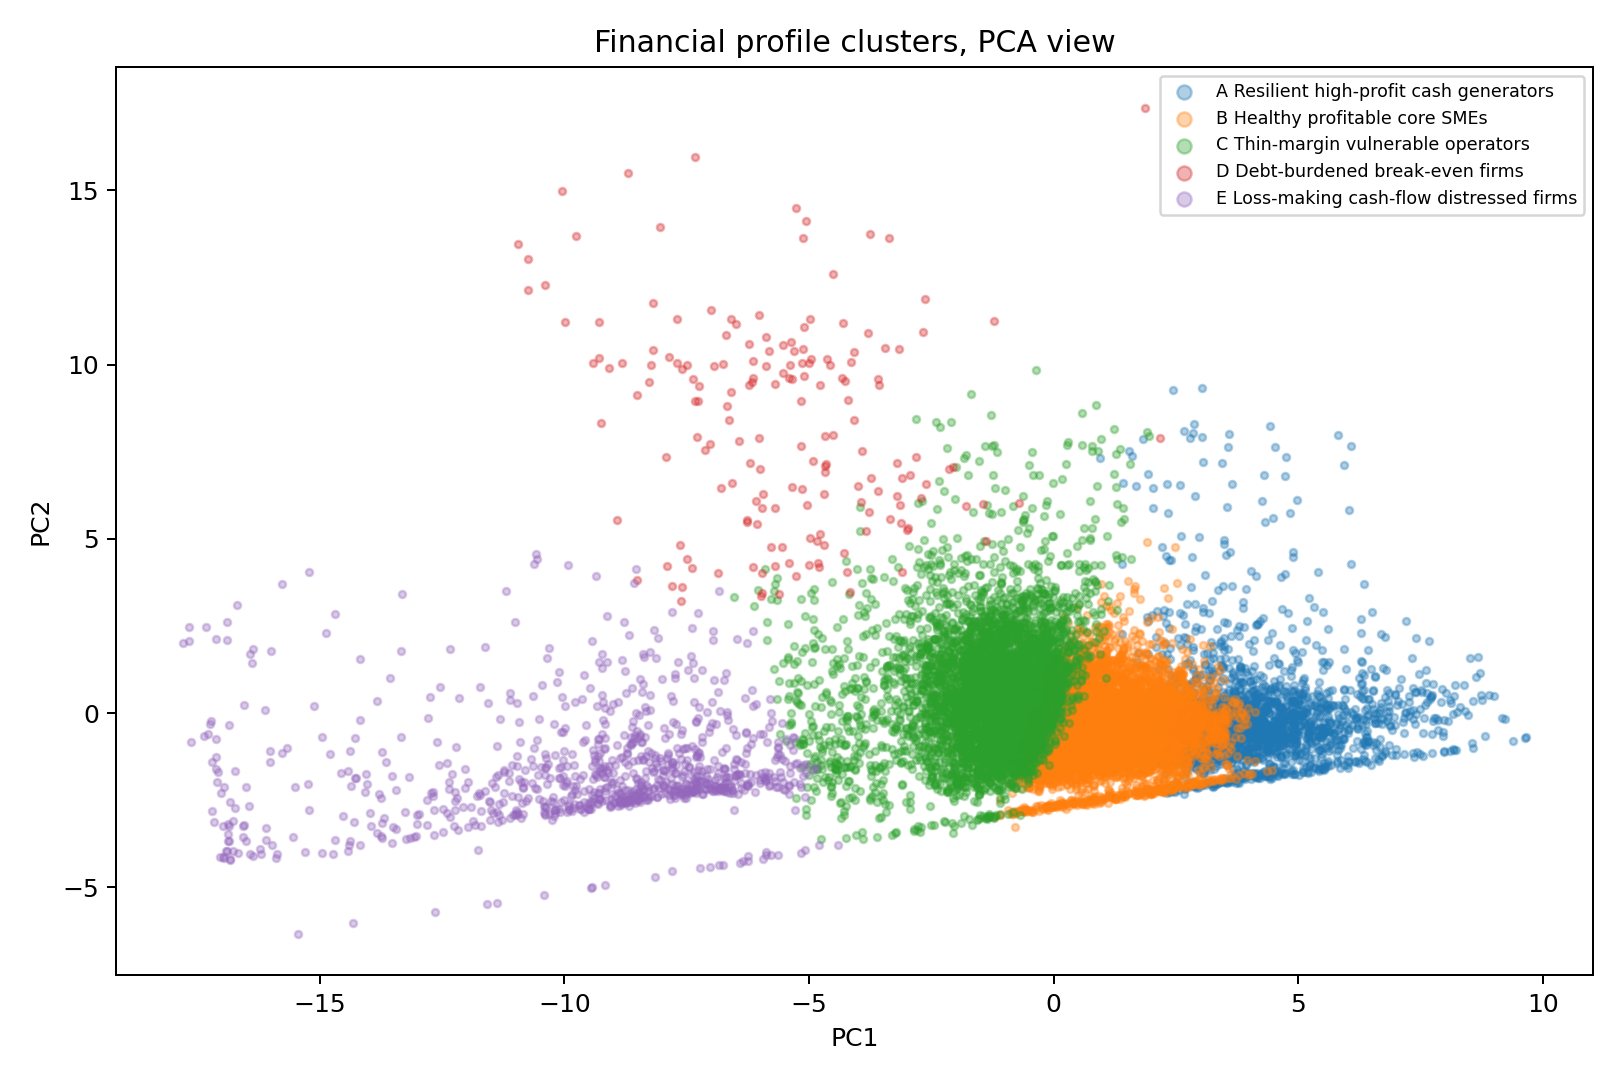
\includegraphics[width=\textwidth]{cluster_pca.png}
    \end{column}
    \begin{column}{0.35\textwidth}
      \scriptsize
      \textbf{PCA components}
      \begin{itemize}
        \item \textbf{PC1 = profitability and cash generation}
        \item Explains \pct{52.7} of scaled variance.
        \item Positive: operating income, cash flow, net margin, operating margin.
        \item Negative: high financial-expense ratios and negative-income flags.
        \item \textbf{PC2 = debt-service pressure}
        \item Explains \pct{14.4} of scaled variance.
        \item Positive: financial expenses relative to sales and operating income.
      \end{itemize}

      \vspace{0.05cm}
      \textbf{Centroids:} A/B are on the healthy PC1 side; C is weaker but central;
      D is high on PC2; E is strongly negative on PC1.
    \end{column}
  \end{columns}
\end{frame}

\begin{frame}{PCA View: Sector Interpretation}
  \begin{columns}[T,totalwidth=\textwidth]
    \begin{column}{0.54\textwidth}
      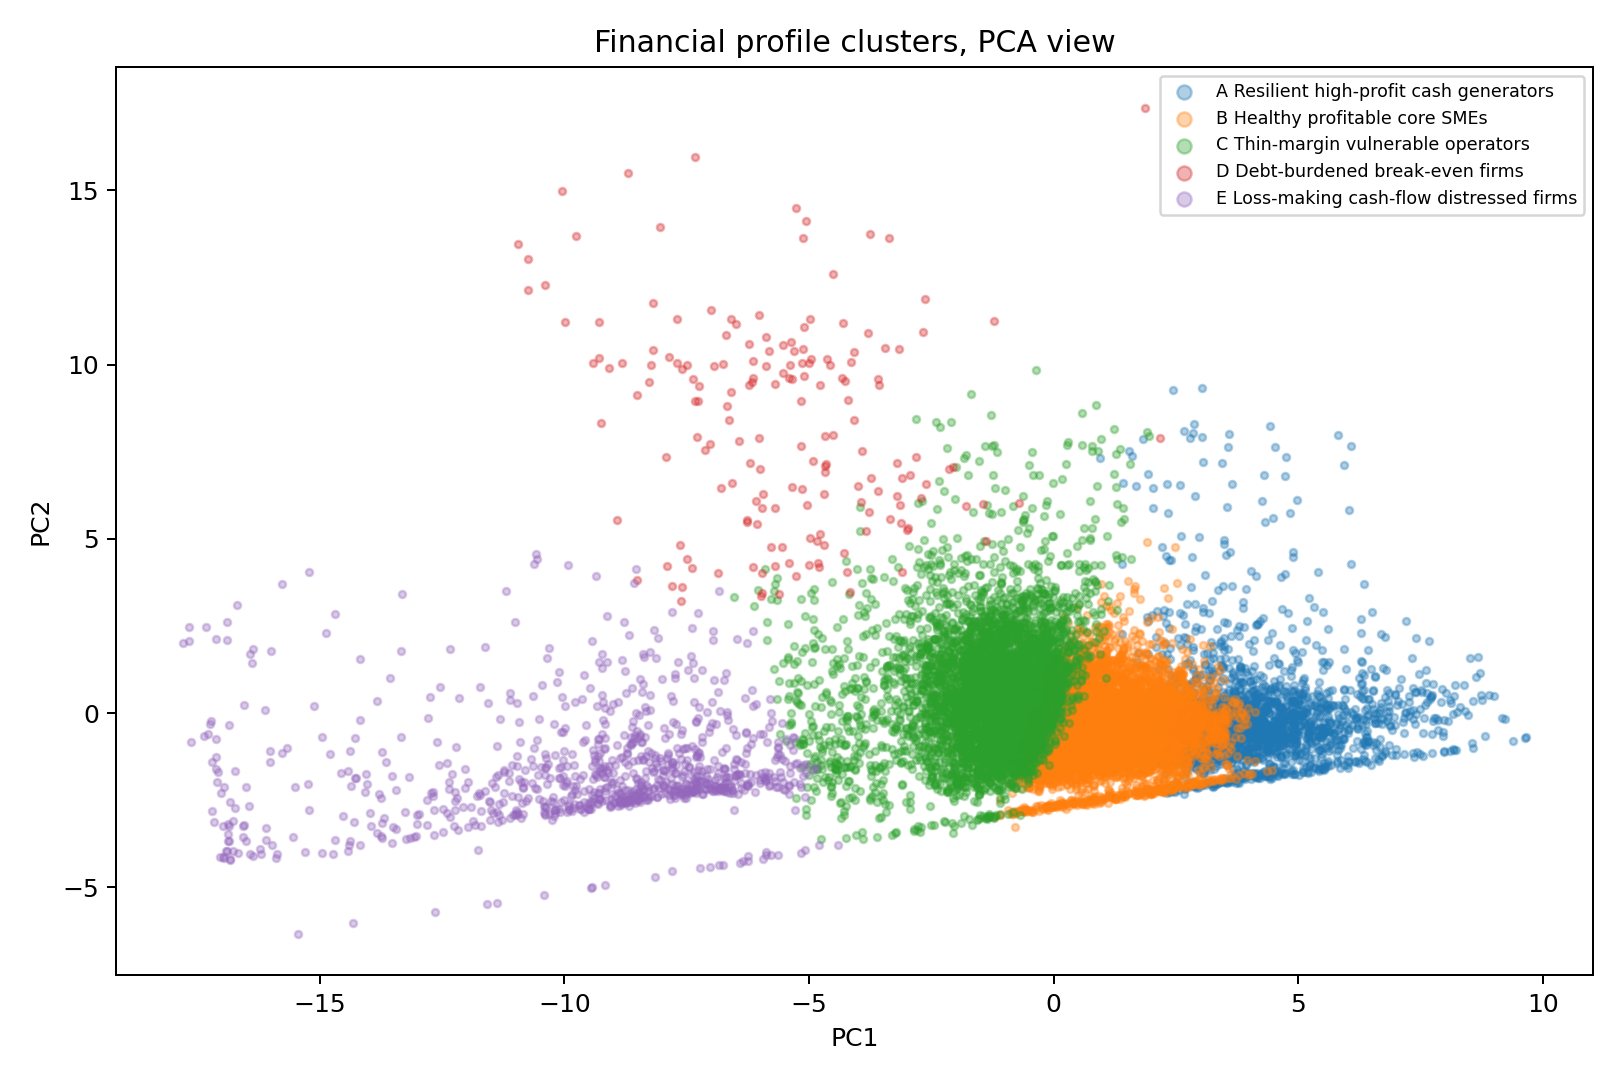
\includegraphics[width=\textwidth]{cluster_pca.png}
    \end{column}
    \begin{column}{0.42\textwidth}
      \scriptsize
      \textbf{Sector lift reading}
      \begin{itemize}
        \item \textbf{A Cash generators:} professional/technical services, health, software, hotels.
        \item \textbf{B Profitable core:} wholesale trade, ICT equipment, machinery and food wholesale.
        \item \textbf{C Thin-margin:} restaurants, food retail, bars, cleaning, motor-vehicle parts.
        \item \textbf{D Debt-burdened:} rubber, printing, beverages, textiles, waste collection.
        \item \textbf{E Loss-making:} R\&D, sports, real estate operations, advertising, leather/textiles.
      \end{itemize}

      \vspace{0.08cm}
      \textbf{Important:} sectors are not clustering inputs. This is a
      post-clustering lift analysis using sectors with at least 30 firms.
    \end{column}
  \end{columns}
\end{frame}

\begin{frame}{Geography of Fragile Profiles}
  \begin{columns}[T,totalwidth=\textwidth]
    \begin{column}{0.62\textwidth}
      \centering
      \includegraphics[height=0.66\textheight,keepaspectratio]{"Regional risk.pdf"}
    \end{column}
    \begin{column}{0.34\textwidth}
      \small
      \textbf{High-risk profiles}
      \begin{itemize}
        \item C: thin-margin vulnerable
        \item D: debt-burdened break-even
        \item E: loss-making cash-flow distressed
      \end{itemize}

      \vspace{0.15cm}
      \begin{tabular}{lr}
        \toprule
        Region & High-risk share \\
        \midrule
        Molise & \pct{51.43} \\
        Lazio & \pct{50.17} \\
        Basilicata & \pct{50.00} \\
        Sicilia & \pct{48.01} \\
        Sardegna & \pct{47.96} \\
        \bottomrule
      \end{tabular}
    \end{column}
  \end{columns}

  \vspace{0.1cm}
  \small
  This is a concentration pattern, not a causal claim about location.
\end{frame}

\begin{frame}{Province-Level Distress Check}
  \begin{columns}[T,totalwidth=\textwidth]
    \begin{column}{0.64\textwidth}
      \centering
      \includegraphics[height=0.70\textheight,keepaspectratio]{"prov distress.pdf"}
    \end{column}
    \begin{column}{0.32\textwidth}
      \small
      \textbf{Target-side view}
      \begin{itemize}
        \item This map shows observed distress rates by province.
        \item It is not used to form the clusters.
        \item It checks whether regional cluster-risk patterns line up with local distress pockets.
      \end{itemize}
    \end{column}
  \end{columns}
\end{frame}

\begin{frame}{Main Takeaways}
  \begin{block}{1. The clusters are economically meaningful}
    The k=5 solution separates SMEs by profitability, cash generation,
    productivity, and debt-service pressure.
  \end{block}

  \begin{block}{2. Distress follows the financial health ladder}
    Distress rises from \pct{0.43} in the strongest cluster to \pct{58.42} in
    the loss-making cash-flow cluster.
  \end{block}

  \begin{block}{3. Geography and sector enrich the interpretation}
    Fragile profiles are not uniformly distributed: some regions and activities
    contain a larger share of thin-margin, debt-burdened, or loss-making firms.
  \end{block}

  \vspace{0.15cm}
  \centering
  \Large \textbf{The clustering turns financial statements into an interpretable risk map.}
\end{frame}

\end{document}
